\chapter{Effetti di inserzione degli strumenti: autoconsumi}

\begin{figure}[h]
    \centering
    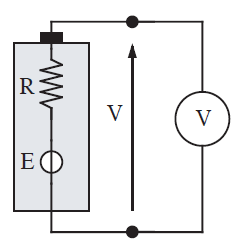
\includegraphics[scale = 1]{Misura reale della tensione.png}
\end{figure}

\newpage 

\section{Inserzione di uno strumento di misura e l'autoconsumo}
\footnote{Slide della prof | SDME Autoconsumi | pag 2 \\  
Appunti | 2025-04-08 | pag 11}

L'inserzione di uno strumento di misura comporta sempre una alterazione delle condizioni del circuito, 
per cui la grandezza sotto misura non è più esattamente quella preesistente. \newline 

L'entità di questa perturbazione deve essere oggetto di attento esame. \newline 

Si consideri, ad esempio, il caso della misura della forza elettromotrice di una pila: 

\begin{figure}[h]
    \centering
    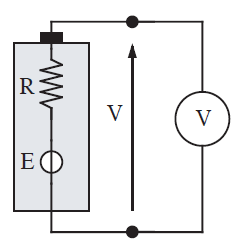
\includegraphics[scale = 0.6]{Misura reale della tensione.png}
\end{figure}


In certe condizioni, l'inserimento del voltmetro può modificare la tensione ai morsetti, che risulta: 


{
    \Large 
    \begin{equation}
        V = E \frac{r}{R + r}
    \end{equation}
}


Considerazioni analoghe possono essere svolte per la misura di una corrente. \newline 

\newpage 

\subsection{Voltmetro a valle}
\footnote{Slide della prof | SDME Autoconsumi | pag 3 \\  
Appunti | 2025-04-08 | pag 12 - 16}

Quando il risultato di una misura dipende dalle indicazioni di due strumenti, 
è necessario considerare gli errori sistematici connessi con il metodo di misura scelto. \newline 

A titolo di esempio, si faccia riferimento allo schema che rappresenta uno dei metodi utilizzabili per determinare la resistenza di un bipolo passivo, 
cioè una misura di resistenza con voltmetro a valle: 

\begin{figure}[h]
    \centering
    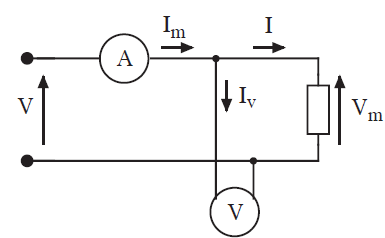
\includegraphics[scale = 0.6]{Misura di resistenza con volmetro a valle.png}
\end{figure}

Visualizzando i resistori dell'amperometro e del voltmetro: 

\begin{figure}[h]
    \centering
    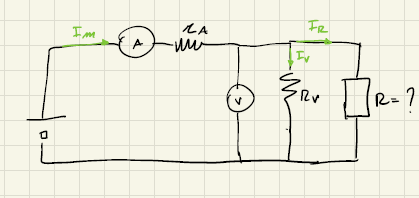
\includegraphics[scale = 0.8]{Misura di resistenza con volmetro a valle schema lezione.png}
\end{figure}

Mentre il voltmetro misura la stessa tensione applicata al bipolo perchè sono in parallelo, 
per questo ultimo motivo l'amperometro misura una corrente che è la somma di quella assorbita dal bipolo e di quella richiesta dal voltmetro. \newline 

Di conseguenza, il rapporto $\frac{V_m}{I_m}$ non rappresenta esattamente il valore di R della grandezza incognita. \newline 

Facendo i conti: 

{
    \Large 
    \begin{equation}
        \begin{split}
            R_m 
            &= 
            \frac{V_m}{I_m}
            \\ 
            &= 
            \frac{V_m}{I + I_v} 
            \\ 
            &= 
            \frac{V_m}{I + \frac{V_m}{R_v}} 
            < 
            \frac{V_m}{I} 
            = 
            R
        \end{split}
    \end{equation}
}

Il metodo usato comporta quindi un errore sistematico in diminuzione, 
attribuile all'autoconsumo del voltmetro. \newline 

Si può assumere:

{
    \Large 
    \begin{equation}
        \begin{split}
            R_m &= R
            \\ 
            &\updownarrow 
            \\ 
            R_v &\to \infty
        \end{split} 
    \end{equation}
}


\newpage 

\subsection{Voltmetro a monte}
\footnote{Slide della prof | SDME Autoconsumi | pag 4 \\  
Appunti | 2025-04-08 | pag 12 - 16}

Svolgendo una misura di resistenza con voltmetro a monte come nel caso in figura: 

\begin{figure}[h]
    \centering
    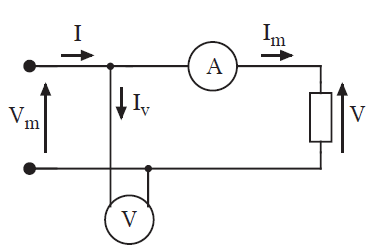
\includegraphics[scale = 0.6]{Misura di resistenza con volmetro a monte.png}
\end{figure}

Visualizzando i resistori dell'amperometro e del voltmetro: 

\begin{figure}[h]
    \centering
    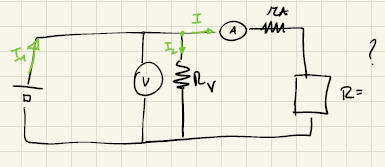
\includegraphics[scale = 0.8]{Misura di resistenza con volmetro a monte schema lezione.png}
\end{figure}

Il rapporto $\frac{V_m}{I_m}$ fornisce un valore $R_m$ in eccesso rispetto a R. \newline 

Facendo i conti: 

{
    \Large 
    \begin{equation}
        \begin{split}
            R_m 
            &= 
            \frac{V_m}{I_m}
            \\ 
            &= 
            \frac{V + r_a I_m}{I_m} > \frac{V}{I_m} = R
        \end{split}
    \end{equation}
}

In questo caso, è l'amperometro che misura esattamente la corrente che circola nel bipolo, 
mentre il voltmetro misura una tensione che è la somma di quella dei morsetti del bipolo aumentata della caduta 
di tensione ai morsetti dell'amperometro. \newline 

Il metodo usato comporta un errore sistematico in aumento. \newline 

Si può assumere: 

{
    \Large 
    \begin{equation}
        \begin{split}
            R_m &= R 
            \\
            &\updownarrow
            \\
            r_a <&< R
        \end{split}
    \end{equation}
}

Trattandosi di errori di tipo sistematico, sia la misura in resistenza con voltmetro a monte che a valle, conoscendo le caratteristiche di autoconsumo 
degli strumenti, cioè la resistenza del voltmetro e dell'amperometro, 
è possibile correggere i risultati della misura finale. \newline 


\newpage 


